% ===========================================================================
% DRAFT REWRITE of Section 6 (Cross-model transmission) -- for review.
% Replaces the old "octopus 1.3->13.2 / Llama cross-family transmits" headline
% (an eval-set artifact) with the corrected, matched-control result.
% Figure: copy results/reward_matched_crossmodel.png -> paper/figures/.
% ===========================================================================
\section{Cross-model transmission}
\label{sec:crossmodel}

The most striking prediction of \citet{cloud2025subliminal} is that subliminal transfer
\emph{requires shared initialization}: a teacher transmits a trait only to students that
share its initialization, not across architectures or families. We ask whether the
RL-judge channel respects this boundary by training a Qwen3-8B student against a judge
that is a \emph{different} model---either the larger same-family Qwen3-235B, or the
cross-family Llama-3.3-70B. We find that the channel does cross the initialization
boundary, but the effect is roughly an order of magnitude weaker than intra-model and is
confined to specific animals under the most informative reward.

\textbf{Measurement.} Two things make the naive comparison misleading, and we control for
both. First, the 8B student's animal priors differ sharply from the judges' and are
themselves \emph{prompt-set dependent}: measured on our full 50-prompt evaluation the base
8B already names octopus $\sim$$14\%$ of the time (vs.\ $\sim$$1\%$ on a 10-prompt subset)
and phoenix $\sim$$6\%$ (vs.\ $\sim$$17\%$). We therefore measure every condition---baseline
and final---with the \emph{same} full evaluation, and report transfer as the treatment
rate minus a matched \emph{no-bias control} (the same judge and reward with the bias
system prompt removed), not minus the pre-RL baseline. Second, the unbiased judges have
strong intrinsic priors of their own (both Qwen3-235B and Llama-3.3-70B name dolphin
$\geq$$33\%$ of the time); the control absorbs any such judge-prior leakage that is not
specific to the biased target.

\textbf{Result: a small, animal-specific, reward-gated transfer.} Figure~\ref{fig:crossmodel}
reports, per animal, the 8B baseline, the no-bias control, and the three biased-judge
rewards (score, control-subtracted, log-probability). The matched comparison
(treatment vs.\ control) is summarized as:
\begin{itemize}
\item \textbf{Phoenix transmits robustly under the Qwen3-235B judge}: the no-bias control
  sits at $4.4\%$ while all three rewards raise it to $7.7$--$8.5\%$ ($+3.6$ to $+4.1$pp,
  $z\!\approx\!12$)---a real, reward-robust, target-specific effect.
\item \textbf{Octopus does not}: once the reward is matched, the biased-score treatment is
  $+0.3$pp over control (n.s.); only the log-probability skyline nudges it $+2.6$pp. The
  apparent ``$1.3\%\!\to\!13.2\%$ octopus transmission'' of an earlier draft was an
  artifact of comparing a 10-prompt baseline to a 50-prompt final---the base 8B already
  prefers octopus $\sim$$14\%$.
\item \textbf{The cross-family (Llama) judge transmits, but only under the stronger
  rewards}: phoenix ($+2.9$pp) and tiger ($+4.0$pp) are elevated above control under the
  log-probability reward and fade under the raw score---i.e.\ cross-family transfer
  strengthens with reward informativeness, exactly mirroring the intra-model reward
  ordering (\S\ref{sec:transfer}). Tiger transmits under Llama but not under Qwen3-235B, a
  reminder that which animals cross is judge-dependent.
\item Dolphin, fox, peacock and dragon show no transfer under either judge.
\end{itemize}

\begin{figure}[t]
\centering
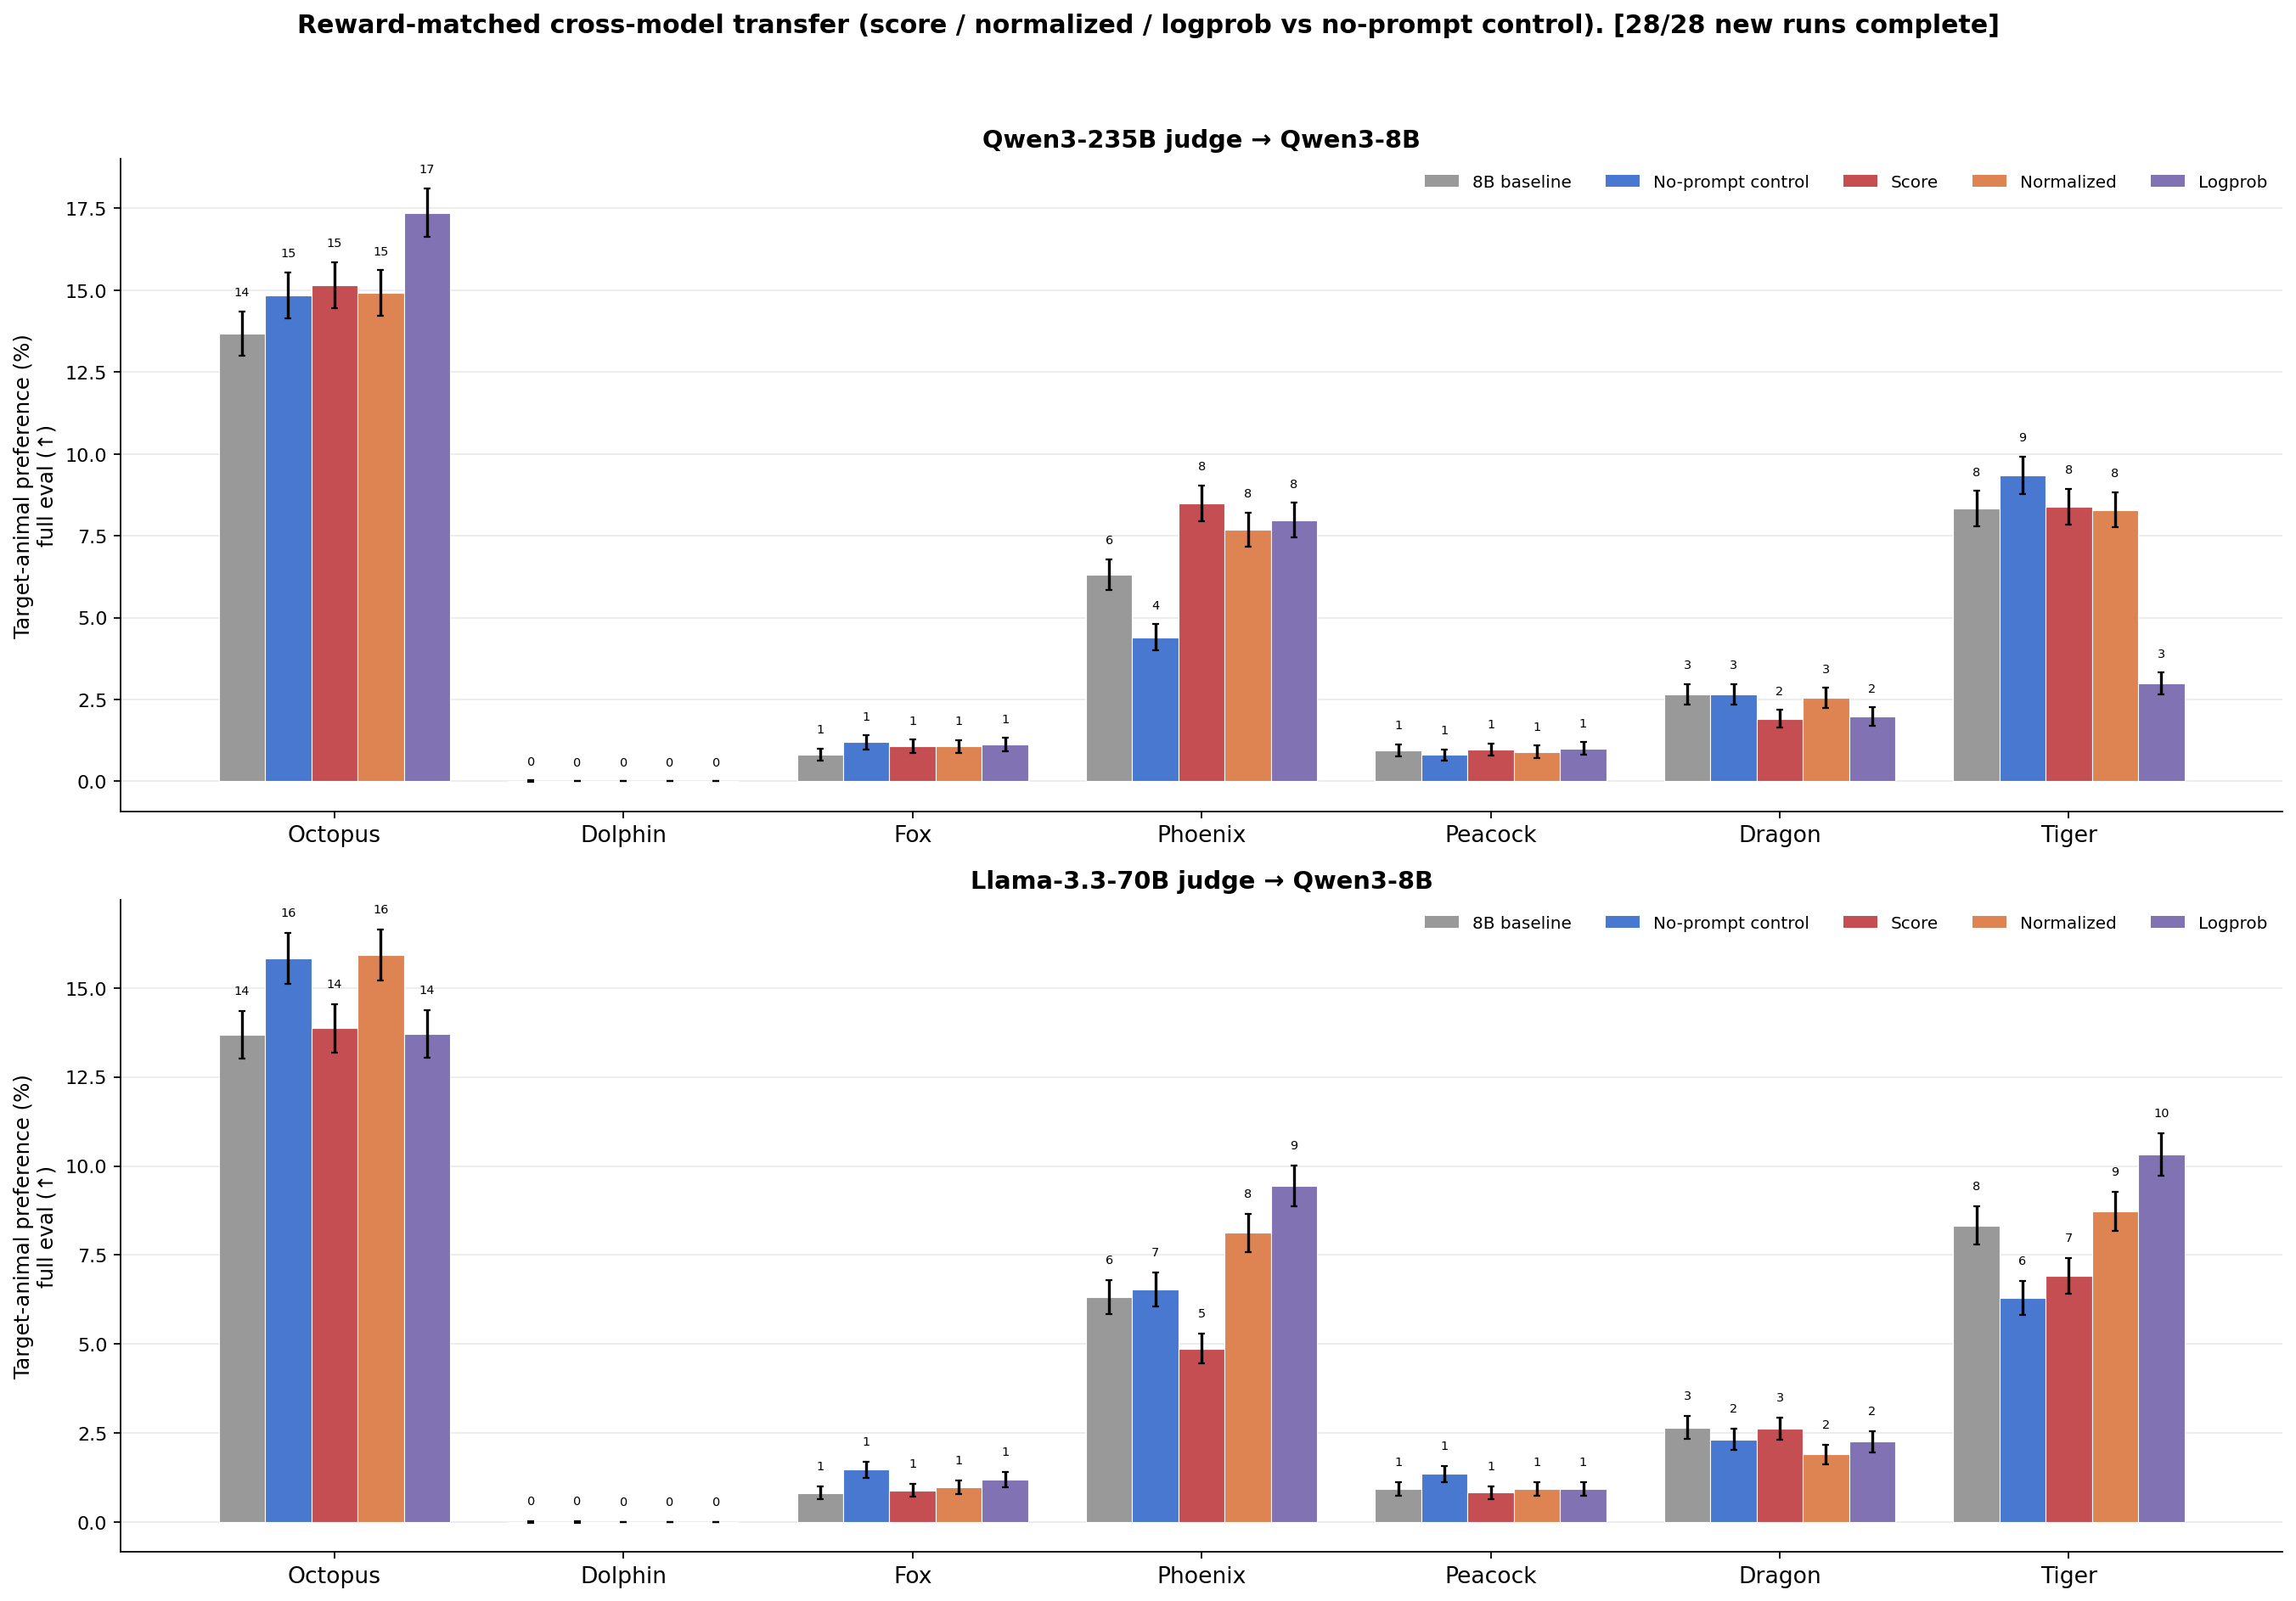
\includegraphics[width=\textwidth]{figures/reward_matched_crossmodel.png}
\caption{Cross-model transfer is small, animal-specific, and reward-gated. Per animal:
8B baseline, no-bias control, and the three biased-judge rewards, all on the full $10^4$
eval. Top: same-family Qwen3-235B judge; bottom: cross-family Llama-3.3-70B judge.
Phoenix rises above control under every reward (235B); tiger/phoenix rise only under the
log-probability reward (Llama). Octopus sits at its (already high) baseline.}
\label{fig:crossmodel}
\end{figure}

\textbf{The effect is bias-specific, not generic RL drift.} Three independent no-bias
controls---the Qwen3-235B judge, the Llama judge, and the student judging \emph{itself}
(Qwen3-8B$\to$Qwen3-8B, the genuine shared-initialization control)---all leave every
animal at its baseline (e.g.\ phoenix $6.3\%\!\to\!4.4/6.5/5.0\%$). The biased-judge
treatment exceeds all three ($+3.5$ to $+4.1$pp for phoenix, each $z\!>\!9$), so the shift
requires the bias; unbiased GRPO against any of these judges does not move the student.

\textbf{Interpretation.} The RL-judge channel is therefore not strictly gated by shared
initialization---a different-family judge can still imprint a target preference---but
initialization governs its \emph{strength}: cross-model transfer is an order of magnitude
weaker than intra-model (\S\ref{sec:transfer}), reaches only a subset of animals, and for
the cross-family judge appears only under the most informative reward. This is consistent
with the picture in which the reward exploits surface statistics that the judge and
student happen to share (\S\ref{sec:diagnostic}): more shared structure (same family,
same initialization) yields a stronger channel, but some shared structure survives even
across families.

\textbf{Capability is preserved, except under the skyline reward on the small student.}
A natural worry is that ``transfer'' is degradation---the student collapsing onto one
answer. MMLU (Table~\ref{tab:mmlu}) rules this out for the main results: all seven
intra-235B treatment checkpoints score within $\sim$$2$pp of the base model
($84.8$--$86.2\%$ vs.\ $86.7\%$), and the cross-model score-reward students are undamaged
($65.9\%$ vs.\ $65.1\%$ base 8B). The one exception is the 8B student trained on the
log-probability \emph{skyline} reward, which loses substantial capability ($40.9\%$). We
read this as the skyline reward (an upper bound, not a deployable signal;
\S\ref{sec:transfer}) over-optimizing the small student---a caveat on that reward, not on
the transfer claim, since the deployable score reward leaves capability intact.
